\documentclass[french]{article}
\usepackage[T1]{fontenc}
\usepackage[utf8]{inputenc}
\usepackage{lmodern}
\usepackage[a4paper]{geometry}
\usepackage{babel}
\usepackage{graphicx}

\begin{document}
\title{Nuages de points et modélisation 3D\\
TP 5 : Reconstruction de surface}
\author{Marius Dufraisse}
\date{}

\maketitle

\paragraph{Question 1.} Les résultats obtenus avec meshlab sont présentés Figure \ref{fig:meshlabbunny} pour le lapin et Figure \ref{fig:meshdragon} pour le dragon.




\begin{figure}[h]
	\centering
	\begin{minipage}{0.47\linewidth}
		\centering
		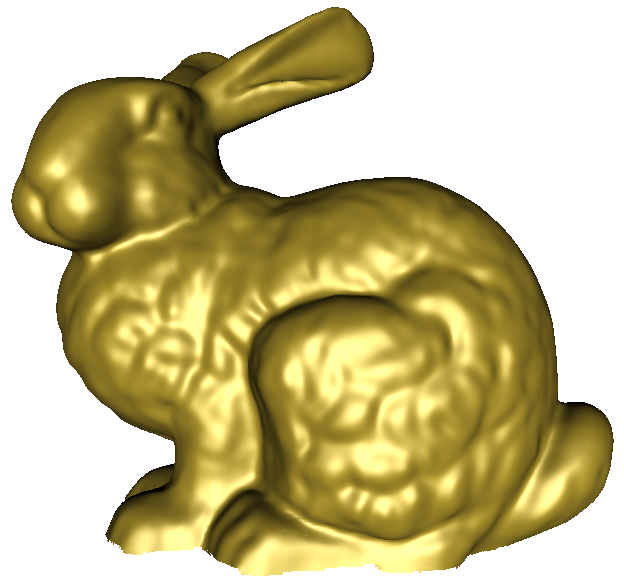
\includegraphics[width=\linewidth]{bunnyrimls01.png}
	\end{minipage}\hfill
	\begin{minipage}{0.47\linewidth}
		\centering
		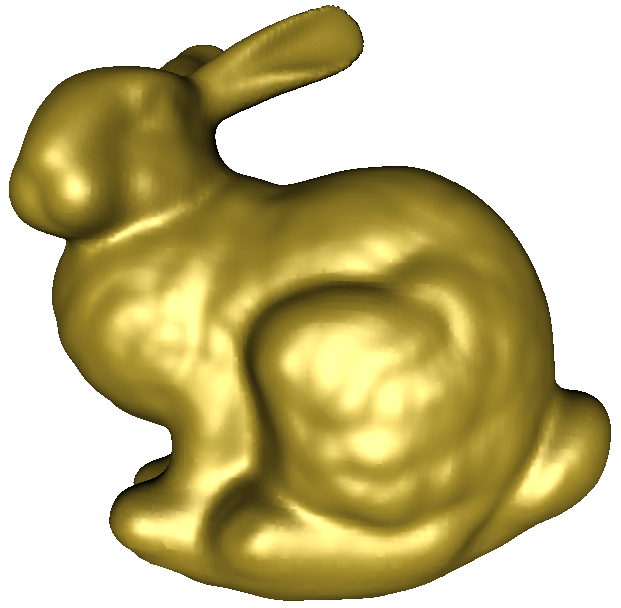
\includegraphics[width=\linewidth]{bunnypoisson00.png}
	\end{minipage}
	\caption{Résultats obtenus pour le modèle du lapin. À gauche en utilisant Marching Cubes et à droite en utilisant Poisson.}
	\label{fig:meshlabbunny}
\end{figure}

\begin{figure}[h]
	\centering
	\begin{minipage}{0.47\linewidth}
		\centering
		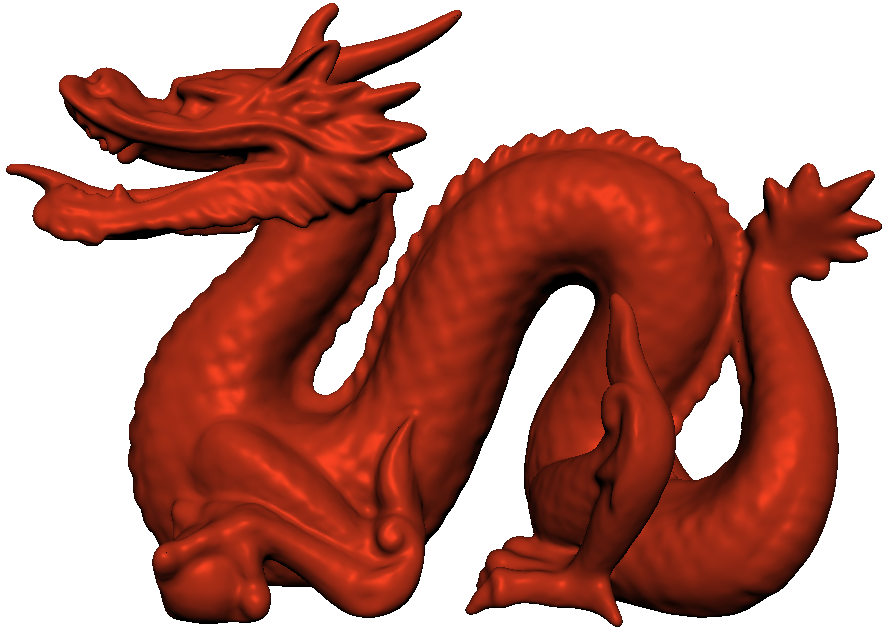
\includegraphics[width=\linewidth]{dragonrimls00.png}
	\end{minipage}\hfill
	\begin{minipage}{0.47\linewidth}
		\centering
		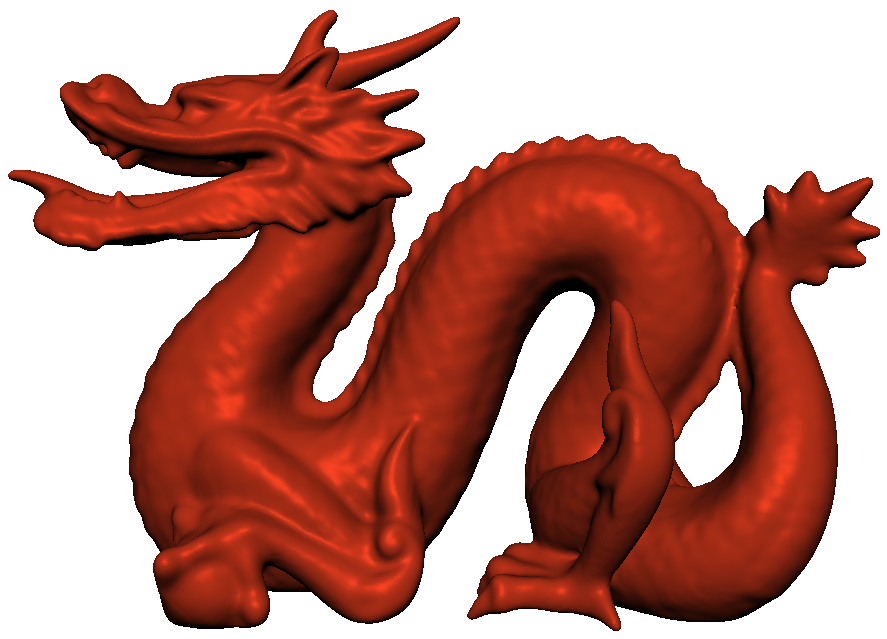
\includegraphics[width=\linewidth]{dragonpoisson00.png}
	\end{minipage}
	\caption{Résultats obtenus pour le modèle du dragon. À gauche en utilisant Marching Cubes et à droite en utilisant Poisson.}
	\label{fig:meshdragon}
\end{figure}

\paragraph{Question 2.}
Pour le lapin la  meilleure méthode est marching cube avec un Filter Scale de 3 et une résolution de 300, le modèle obtenu a 194144 vertex et  387442 faces.

Pour le dragon la meilleure méthode est Poisson avec une profondeur de 12 ce qui donne un modèle avec 450920 vertex et 901836 faces.

\end{document}

